\chapter{Percobaan Awal}
\label{chap:percobaan_awal}
Pada bab ini akan dijelaskan analisis masalah penelitian ini. Analisis meliputi Eksplorasi Teknologi, Dataset Pada HTTP Archive, Langkah-Langkah Query Yang Dilakukan, dan Hasil Sample Data Dengan Beberapa Aplikasi.

\section{Eksplorasi Teknologi}
Dalam pengerjaan skripsi ini akan menggunakan teknologi bernama BigQuery. Di dalam BigQuery, terdapat salah satu fitur yang akan digunakan yaitu membuat dataset baru. Dataset bisa saja diambil dari public dataset maupun membuat sendiri datasettersbut. Dataset berisi tabel-tabel yang akan dianalisis. Tabel-tabel tersebut dapat dibuat secara manual maupun di-\textit{upload}.

Berikut ini langkah-langkah dalam pembuatan dataset dan tabel:
\begin{enumerate}
	\item Membuka Google Cloud Project Page\footnote{https://console.cloud.google.com/getting-started}. Halaman yang akan ditampilkan dapat dilihat pada gambar \ref{fig:GCP}
	\begin{figure}[H]
		\centering  
		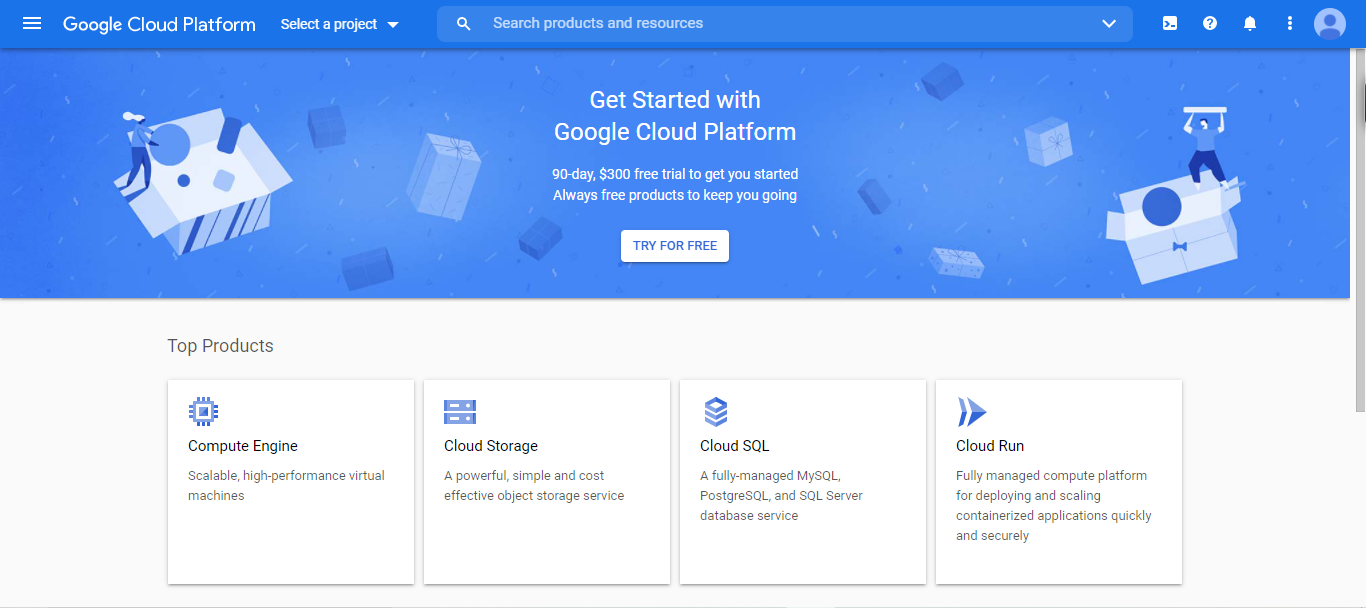
\includegraphics[scale=0.45]{Gambar/open_GCP.PNG}  
		\caption{Google Cloud Project Page} 
		\label{fig:GCP} 
	\end{figure}
	\item Membuat atau memilih \textit{project} yang akan dikerjakan. Halaman yang akan ditampilkan dapat dilihat pada gambar \ref{fig:create_or_open}
	\begin{figure}[H]
		\centering  
		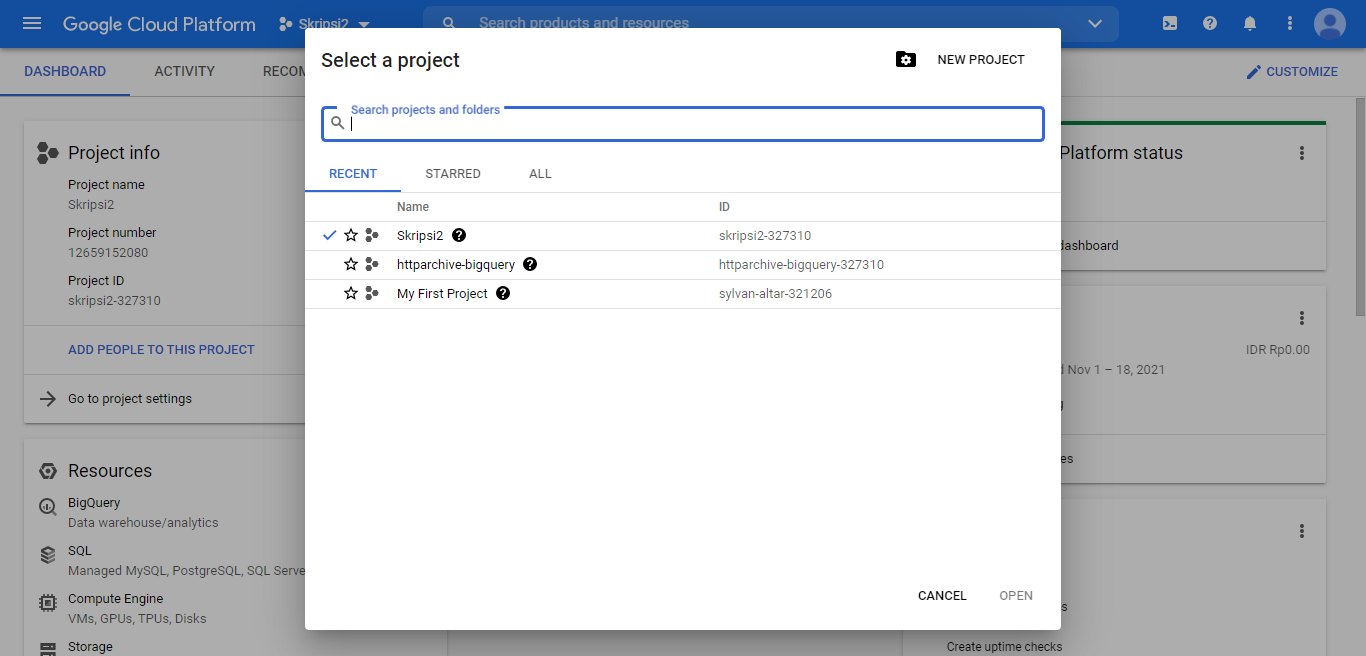
\includegraphics[scale=0.45]{Gambar/pilih_project.PNG}  
		\caption{Create atau Open Project} 
		\label{fig:create_or_open} 
	\end{figure}
	\item Membuka \textit{console} kemudian memilih BigQuery. Halaman yang akan ditampilkan dapat dilihat pada gambar \ref{fig:BQ}
	\begin{figure}[H]
		\centering  
		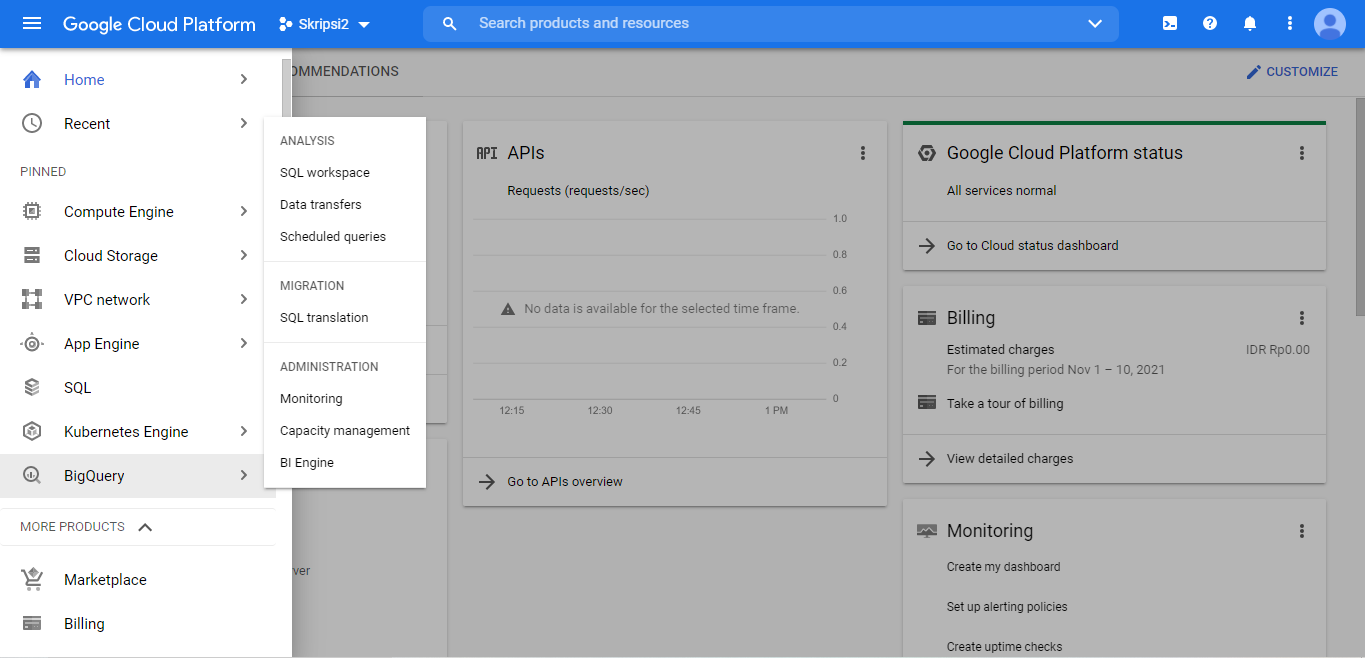
\includegraphics[scale=0.45]{Gambar/console_BigQuery.PNG}  
		\caption{Membuka BigQuery} 
		\label{fig:BQ} 
	\end{figure}
	\item Pada tab explorer terdapat project kemudian pengguna harus menekan tombol titik tiga dan piliih \textit{create} dataset. Halaman yang akan ditampilkan dapat dilihat pada gambar \ref{fig:create_dataset}
	\begin{figure}[H]
		\centering  
		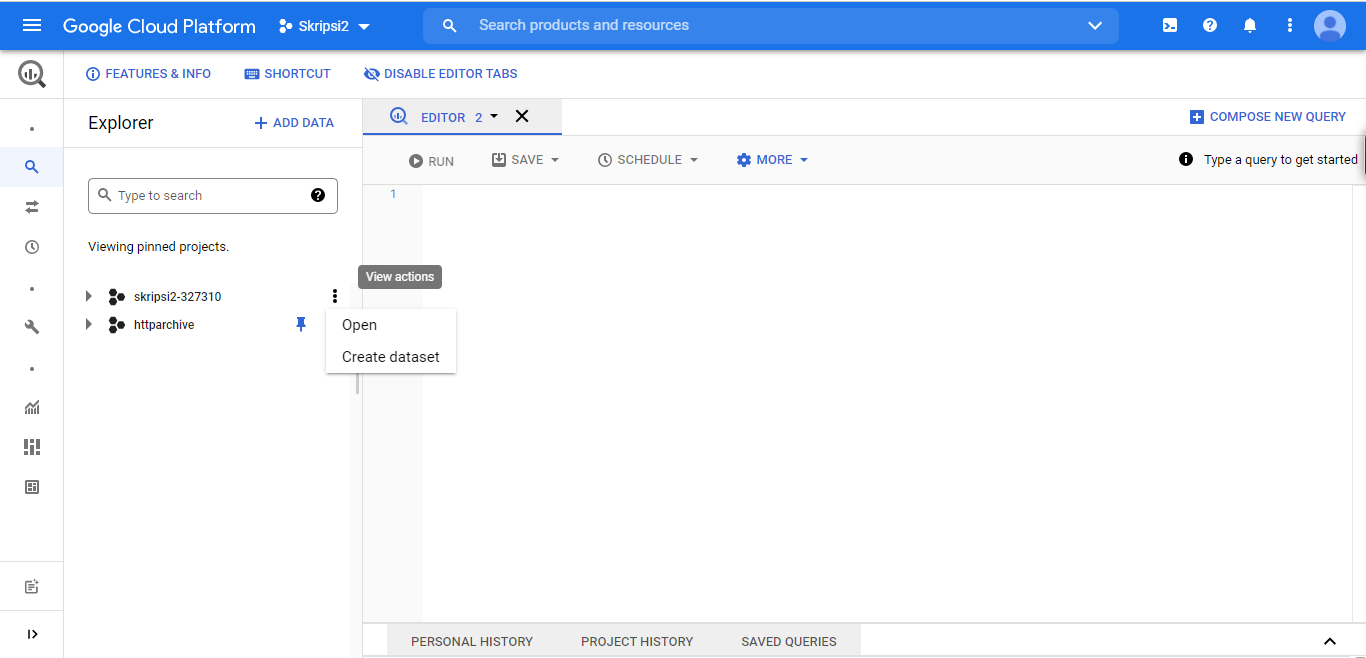
\includegraphics[scale=0.45]{Gambar/create_dataset.PNG}  
		\caption{Membuat Dataset Baru} 
		\label{fig:create_dataset} 
	\end{figure}
	\item Buka dataset, kemudian pilih menu \textit{create table}. Halaman yang akan ditampilkan dapat dilihat pada gambar \ref{fig:create_table}
	\begin{figure}[H]
		\centering  
		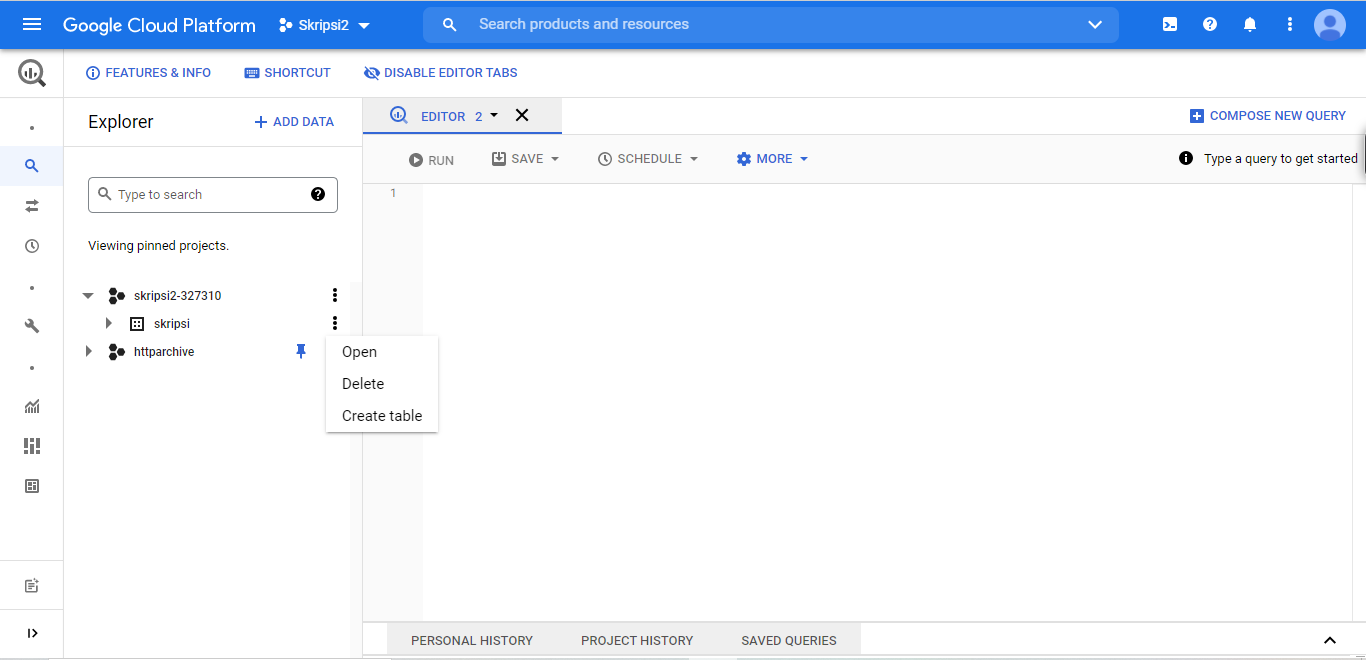
\includegraphics[scale=0.45]{Gambar/create_table.PNG}  
		\caption{Membuat Tabel Baru} 
		\label{fig:create_table} 
	\end{figure}
\end{enumerate}

\section{Dataset Pada HTTP Archive}
Dataset pada HTTP Archive yang digunakan pada skripsi ini adalah sebagai berikut:
\begin{enumerate}
	\item technologies
	Pada tabel technologies terdapat beberapa kolom seperti url, category, app, dan info. Url adalah alamat dari sebuah website. Contoh dari dataset dapat dilihat pada tabel \ref{table:ct_tech_desktop} 
	\begin{table}[H]
		\centering
		\begin{tabular}{|l|l|p{3cm}|p{3cm}|l|}
			\hline
			\textbf{Row} & \textbf{url} & \textbf{category} & app & info\\
			\hline
			1 & https://www.3-king.com/ & Analytics & Google Analytics & \\
			\hline
			2 & https://www.fleabites.net/ & Miscellaneous & Twitter Emoji (Twemoji) & \\
			\hline
			3 & http://www.elcarnicero.cl/ & Widgets & OWL Carousel & \\
			\hline
			4 & https://thankyou.ws/ & Analytics & Google Analytics & \\
			\hline
			5 & https://rogerwaters.com/ & Reverse proxies & Nginx & \\
			\hline
			6 & http://www.palaciodaslampadas.com.br/ & JavaScript libraries & jQuery & 2.1.1\\
			\hline
			7 & https://copenhagencamping.dk/ & CMS & WordPress & \\
			\hline
			8 & https://eachat.ma/ & Ecommerce & WooCommerce & 4.3.0\\
			\hline
			9 & https://advokat-bondarchuk.ru/ & Blogs & WordPress & \\
			\hline
			10 & https://passport.rsl.ru/ & JavaScript libraries & jQuery & 1.7.1\\
			\hline
		\end{tabular}
		\caption{Technologies Desktop Data Sample}
		\label{table:ct_tech_desktop}
	\end{table}
	
	
	
\end{enumerate}
Di dalam HTTP Archive terdapat dataset yang dapat diambil menggunakan teknologi BigQuery. Dataset dari HTTP Archive masih kotor sehingga terdapat beberapa data yang ganda dan terdapat versi dari aplikasi yang tidak valid (hanya berisi karakter atau simbol). Dataset tersebut adalah sebagai berikut:
\begin{enumerate}
	\item almanac\\
	Pada tabel ini tidak terdapat keterangan dan tidak berhubungan dengan skripsi ini.
	\item blink$\_$features\\
	Pada tabel ini tidak terdapat keterangan dan tidak berhubungan dengan skripsi ini.
	\item core$\_$web$\_$vitals\\
	Pada tabel ini tidak terdapat keterangan dan tidak berhubungan dengan skripsi ini.
	\item latest\\
	Pada tabel ini tidak terdapat keterangan dan tidak berhubungan dengan skripsi ini.
	\item lighthouse\\
	Dataset pada lighthouse berisi tabel-tabel dari bulan Juni tahun 2017 sampai dengan sekarang yang terdiri dari website pada mobile. Dataset bulan Agustus tahun 2020 baris pada mobile memiliki 6.290.147 baris.Contoh data dapat dilihat pada tabel \ref{table:ct_lh_mobile}. Tabel terdiri dari url dan report. \textit{URL (Uniform Resource Locator)} merupakan nama-nama domain dan \textit{report}. Tetapi tabel ini tidak digunakan dalam pengerjaan skripsi ini. 
	
	
	\begin{table}[H]
		\centering
		\begin{tabular*}{\textwidth}{|l|p{14.4cm}|}
			\hline
			\textbf{url} & \url{https://votesearch.utah.gov/}\\ 
			\hline
			\textbf{report} & \{"userAgent":"Mozilla/5.0 (X11; Linux x86\_64) AppleWebKit/537.36 (KHTML, like Gecko) Chrome/84.0.4147.105 Safari/537.36","environment":\{"networkUserAgent": "Mozilla/5.0 (Linux; Android 7.0; Moto G (4)) AppleWebKit/537.36 (KHTML, like Gecko) Chrome/84.0.4143.7 Mobile Safari/537.36 Chrome-Lighthouse","hostUserAgent":"Mozilla/5.0 (X11; Linux x86\_64) AppleWebKit/537.36 (KHTML, like Gecko) Chrome/84.0.4147.105 Safari/537.36","benchmarkIndex":506\},"lighthouseVersion": "6.1.1" ,"fetchTime": "2020-08-06T10:36:03.335Z" ,"requestedUrl":"\url{https://votesearch.utah.gov/}","finalUrl":"\url{https://vote.utah.gov/}","runWarnings":["The page may not be loading as expected because your test URL (\url{https://votesearch.utah.gov/}) was redirected to https://vote.utah.gov/. Try testing the second URL directly."],"audits":\{"is-on-https":\{"id":"is-on-https","title":"Does not use HTTPS","description":"All sites should be protected with HTTPS, even ones that don't handle sensitive data. This includes avoiding [mixed content](\url{https://developers.google.com}...\\
			\hline
			
		\end{tabular*}
		\caption{Lighthouse Data Example}
		\label{table:ct_lh_mobile}
	\end{table}
	
	% \begin{sidewaystable} % <-- HERE
		% \centering
		% \begin{tabular}{|l|l|@{\extracolsep{\fill}}p{18cm}|}\hline
			% 1 & \url{https://votesearch.utah.gov/} & \{"userAgent":"Mozilla/5.0 (X11; Linux x86\_64) AppleWebKit/537.36 (KHTML, like Gecko) Chrome/84.0.4147.105 Safari/537.36","environment":\{"networkUserAgent": "Mozilla/5.0 (Linux; Android 7.0; Moto G (4)) AppleWebKit/537.36 (KHTML, like Gecko) Chrome/84.0.4143.7 Mobile Safari/537.36 Chrome-Lighthouse","hostUserAgent":"Mozilla/5.0 (X11; Linux x86\_64) AppleWebKit/537.36 (KHTML, like Gecko) Chrome/84.0.4147.105 Safari/537.36","benchmarkIndex":506\},"lighthouseVersion": "6.1.1" ,"fetchTime": "2020-08-06T10:36:03.335Z" ,"requestedUrl":"\url{https://votesearch.utah.gov/}","finalUrl":"\url{https://vote.utah.gov/}","runWarnings":["The page may not be loading as expected because your test URL (\url{https://votesearch.utah.gov/}) was redirected to https://vote.utah.gov/. Try testing the second URL directly."],"audits":\{"is-on-https":\{"id":"is-on-https","title":"Does not use HTTPS","description":"All sites should be protected with HTTPS, even ones that don't handle sensitive data. This includes avoiding [mixed content](\url{https://developers.google.com}...\\
			% \hline
			% \end{tabular}
		% \caption{Lighthouse Data Example}
		% \label{table:ct_lh_mobile}
		% \end{sidewaystable} % <-- HERE
	
	
	%     \begin{table}[H]
		% \centering
		% \begin{tabular*}{\textwidth}{|l|l|@{\extracolsep{\fill}}p{8.8cm}|}
			%  \hline
			%  \textbf{Row} & \textbf{url} & \textbf{report}\\
			%  \hline
			% 1 & \url{https://votesearch.utah.gov/} & \{"userAgent":"Mozilla/5.0 (X11; Linux x86\_64) AppleWebKit/537.36 (KHTML, like Gecko) Chrome/84.0.4147.105 Safari/537.36","environment":\{"networkUserAgent": "Mozilla/5.0 (Linux; Android 7.0; Moto G (4)) AppleWebKit/537.36 (KHTML, like Gecko) Chrome/84.0.4143.7 Mobile Safari/537.36 Chrome-Lighthouse","hostUserAgent":"Mozilla/5.0 (X11; Linux x86\_64) AppleWebKit/537.36 (KHTML, like Gecko) Chrome/84.0.4147.105 Safari/537.36","benchmarkIndex":506\},"lighthouseVersion": "6.1.1" ,"fetchTime": "2020-08-06T10:36:03.335Z" ,"requestedUrl":"\url{https://votesearch.utah.gov/}","finalUrl":"\url{https://vote.utah.gov/}","runWarnings":["The page may not be loading as expected because your test URL (\url{https://votesearch.utah.gov/}) was redirected to https://vote.utah.gov/. Try testing the second URL directly."],"audits":\{"is-on-https":\{"id":"is-on-https","title":"Does not use HTTPS","description":"All sites should be protected with HTTPS, even ones that don't handle sensitive data. This includes avoiding [mixed content](\url{https://developers.google.com}...\\
			% \hline
			% 2 & \url{https://otricolore.ru/} & \{"userAgent": "Mozilla/5.0 (X11; Linux x86\_64) AppleWebKit/537.36 (KHTML, like Gecko) Chrome/84.0.4147.125 Safari/537.36","environment":\{"networkUserAgent": "Mozilla/5.0 (Linux; Android 7.0; Moto G (4)) AppleWebKit/537.36 (KHTML, like Gecko) Chrome/84.0.4143.7 Mobile Safari/537.36 Chrome-Lighthouse","hostUserAgent": "Mozilla/5.0 (X11; Linux x86\_64) AppleWebKit/537.36 (KHTML, like Gecko) Chrome/84.0.4147.125 Safari/537.36","benchmarkIndex":456},"lighthouseVersion": "6.2.0" ,"fetchTime":"2020-08-11T09:30:51.743Z", "requestedUrl": "\url{https://otricolore.ru/}", "finalUrl": "\url{https://otricolore.ru/}","runWarnings":[],"audits":\{"is-on-https":\{"id":"is-on-https","title":"Uses HTTPS","description":"All sites should be protected with HTTPS, even ones that don't handle sensitive data. This includes avoiding [mixed content](\url{https://developers.google.com/web/fundamentals/security/prevent-mixed-content/what-is-mixed-content}), where some resources are loaded over HTTP despite the initial request being servedover HTTPS. HTTPS prevents int…\\
		% \hline
		% \end{tabular*}
	% \caption{Lighthouse Data Example}
	% \label{table:ct_lh_mobile}
	% \end{table}

\item pages\\
Dataset pada pages berisi tabel-tabel dari bulan Januari tahun 2016 sampai dengan sekarang yang terdiri dari website pada desktop dan mobile. Dataset bulan Agustus tahun 2020 baris pada desktop memiliki 5.593.642 baris dan pada mobile memiliki 6.347.640 baris. Contoh data dapat dilihat pada tabel \ref{table:pages_data_sample}.
Masing-masing terdiri dari url dan payload. \textit{URL (Uniform Resource Locator)} merupakan nama-nama domain dan \textit{payload}. Tetapi tabel ini tidak digunakan dalam pengerjaan skripsi ini.

\begin{table}[H]
	\centering
	\begin{tabular*}{\textwidth}{|l|p{14.13cm}|}
		\hline
		\textbf{url} & \url{https://tutorinmobiliario.cl/}\\ 
		\hline
		\textbf{payload} & \{"startedDateTime":"2020-08-14T17:45:37.606+00:00", "title": "Run 1, First View for \url{https://tutorinmobiliario.cl/}", "id": "page\_1\_0\_1", "pageTimings": \{"onLoad":27048,"onContentLoad":-1, "\_startRender":6500\}, "\_cpu.BlinkGC.LazySweepInIdle":10, "\_testStartOffset":0,"\_start\_epoch":0, "\_cpu.ParseAuthorStyleSheet":95,"\_bytesOutDoc": 208779, "\_cpu.V8.GC\_MC\_CLEAR\_STRING\_TABLE":1, "\_cpu.V8.GC\_SCAVENGER\_SCAVENGE\_UPDATE \_REFS": 0, "\_cpu.V8.GC\_MC\_MARK\_EMBEDDER\_TRACING\_CLOSURE":0, "\_cpu.V8.GC\_MC\_MARK\_FINISH\_INCREMENTAL": 0, "\_firstPaint":6445.524999995541, "\_cpu.BlinkGC.AtomicPauseMarkEpilogue":0,  "\_cpu.V8.GC\_MC\_INCREMENTAL\_EMBEDDER \_PROLOGUE":7, "\_cpu.V8.GC\_SCAVENGER\_COMPLETE\_SWEEP\_ARRAY\_BUFFERS":0, "\_cpu.V8.GC\_MC\_EVACUATE\_REBALANCE":0,"\_optimization\_checked":1, "\_cpu.V8.GC\_MC\_MARK\_ROOTS":0, "\_cpu.BlinkGC. IncrementalMarkingStartMarking": 4, "\_responses\_404":0, "\_URL": "\url{https://tutorinmobiliario.cl/}", "\_cpu.V8.GC\_SCAVENGER\_SCAVENGE\_ROOTS":3, "\_loadEventStart":27048, "\_cpu.EvaluateScript":452 , "\_score\_gzip":100, "\_cpu.V8.GC\_MC\_MARK\_WEAK\_CLOSURE\_EPHEMERON\_…\\
		\hline
		
	\end{tabular*}
	\caption{Pages Data Example}
	\label{table:pages_data_sample}
\end{table}

%     \begin{sidewaystable} % <-- HERE
	% \centering
	% \begin{tabular}{|l|l|@{\extracolsep{\fill}}p{18cm}|}\hline
		% 1 & https://tutorinmobiliario.cl/ & \{"startedDateTime":"2020-08-14T17:45:37.606+00:00", "title": "Run 1, First View for \url{https://tutorinmobiliario.cl/}", "id": "page\_1\_0\_1", "pageTimings": \{"onLoad":27048,"onContentLoad":-1, "\_startRender":6500\}, "\_cpu.BlinkGC.LazySweepInIdle":10, "\_testStartOffset":0,"\_start\_epoch":0, "\_cpu.ParseAuthorStyleSheet":95,"\_bytesOutDoc": 208779, "\_cpu.V8.GC\_MC\_CLEAR\_STRING\_TABLE":1, "\_cpu.V8.GC\_SCAVENGER\_SCAVENGE\_UPDATE \_REFS": 0, "\_cpu.V8.GC\_MC\_MARK\_EMBEDDER\_TRACING\_CLOSURE":0, "\_cpu.V8.GC\_MC\_MARK\_FINISH\_INCREMENTAL": 0, "\_firstPaint":6445.524999995541, "\_cpu.BlinkGC.AtomicPauseMarkEpilogue":0,  "\_cpu.V8.GC\_MC\_INCREMENTAL\_EMBEDDER \_PROLOGUE":7, "\_cpu.V8.GC\_SCAVENGER\_COMPLETE\_SWEEP\_ARRAY\_BUFFERS":0, "\_cpu.V8.GC\_MC\_EVACUATE\_REBALANCE":0,"\_optimization\_checked":1, "\_cpu.V8.GC\_MC\_MARK\_ROOTS":0, "\_cpu.BlinkGC.IncrementalMarkingStartMarking":4, "\_responses\_404":0, "\_URL": "https://tutorinmobiliario.cl/", "\_cpu.V8.GC\_SCAVENGER\_SCAVENGE\_ROOTS":3, "\_loadEventStart":27048, "\_cpu.EvaluateScript":452 , "\_score\_gzip":100, "\_cpu.V8.GC\_MC\_MARK\_WEAK\_CLOSURE\_EPHEMERON\_…\\
		% \hline
		% \end{tabular}
	% \caption{Pages Data Sample}
	% \label{table:pages_data_sample}
	% \end{sidewaystable} % <-- HERE

%     \begin{table}[H]
	% \centering
	% \begin{tabular*}{\textwidth}{|l|l|@{\extracolsep{\fill}}p{8.8cm}|}
		%  \hline
		%  \textbf{Row} & \textbf{url} & \textbf{payload}\\
		%  \hline
		% 1 & https://tutorinmobiliario.cl/ & \{"startedDateTime":"2020-08-14T17:45:37.606+00:00", "title": "Run 1, First View for \url{https://tutorinmobiliario.cl/}", "id": "page\_1\_0\_1", "pageTimings": \{"onLoad":27048,"onContentLoad":-1, "\_startRender":6500\}, "\_cpu.BlinkGC.LazySweepInIdle":10, "\_testStartOffset":0,"\_start\_epoch":0, "\_cpu.ParseAuthorStyleSheet":95,"\_bytesOutDoc": 208779, "\_cpu.V8.GC\_MC\_CLEAR\_STRING\_TABLE":1, "\_cpu.V8.GC\_SCAVENGER\_SCAVENGE\_UPDATE\_REFS": 0, "\_cpu.V8.GC\_MC\_MARK\_EMBEDDER\_TRACING\_CLOSURE":0, "\_cpu.V8.GC\_MC\_MARK\_FINISH\_INCREMENTAL": 0, "\_firstPaint":6445.524999995541, "\_cpu.BlinkGC.AtomicPauseMarkEpilogue":0,  "\_cpu.V8.GC\_MC\_INCREMENTAL\_EMBEDDER\_PROLOGUE":7, "\_cpu.V8.GC\_SCAVENGER\_COMPLETE\_SWEEP\_ARRAY\_BUFFERS":0, "\_cpu.V8.GC\_MC\_EVACUATE\_REBALANCE":0,"\_optimization\_checked":1, "\_cpu.V8.GC\_MC\_MARK\_ROOTS":0, "\_cpu.BlinkGC.IncrementalMarkingStartMarking":4, "\_responses\_404":0, "\_URL": "https://tutorinmobiliario.cl/", "\_cpu.V8.GC\_SCAVENGER\_SCAVENGE\_ROOTS":3, "\_loadEventStart":27048, "\_cpu.EvaluateScript":452 , "\_score\_gzip":100, "\_cpu.V8.GC\_MC\_MARK\_WEAK\_CLOSURE\_EPHEMERON\_…\\
		% \hline
		% 2 & https://nishinatoshiharu.com/ & \{"startedDateTime":"2020-08-18T21:50:57.272+00:00","title":"Run 1, First View for https://nishinatoshiharu.com/","id":"page$\_$1$\_$0$\_$1","pageTimings":\{"onLoad":24788,"onContentLoad":-1,"$\_$startRender":4800\},"$\_$cpu.BlinkGC.LazySweepInIdle":28,"$\_$testStartOffset":0,"$\_$start$\_$epoch":0,"$\_$cpu.ParseAuthorStyleSheet":98,"$\_$bytesOutDoc":469240,"$\_$cpu.V8.GC$\_$MC$\_$CLEAR$\_$STRING$\_$TABLE":1,"$\_$cpu.V8.GC$\_$SCAVENGER$\_$SCAVENGE$\_$UPDATE$\_$REFS":0,"$\_$cpu.V8.GC$\_$MC$\_$MARK$\_$EMBEDDER$\_$TRACING$\_$CLOSURE":0,"$\_$cpu.V8.GC$\_$MC$\_$MARK$\_$FINISH$\_$INCREMENTAL":0,"$\_$firstPaint":4826.009999997041,"$\_$cpu.BlinkGC.AtomicPauseMarkEpilogue":0,"$\_$cpu.V8.GC$\_$MC$\_$INCREMENTAL$\_$EMBEDDER$\_$PROLOGUE":14,"$\_$cpu.V8.GC$\_$SCAVENGER$\_$COMPLETE$\_$SWEEP$\_$ARRAY$\_$BUFFERS":0,"$\_$cpu.V8.GC$\_$MC$\_$EVACUATE$\_$REBALANCE":0,"$\_$optimization$\_$checked":1,"$\_$cpu.V8.GC$\_$MC$\_$MARK$\_$ROOTS":0,"$\_$cpu.BlinkGC.IncrementalMarkingStartMarking":9,"$\_$responses$\_$404":0,"$\_$URL":"https://nishinatoshiharu.com/","$\_$cpu.V8.GC$\_$SCAVENGER$\_$SCAVENGE$\_$ROOTS":5,"$\_$loadEventStart":24788,"$\_$cpu.EvaluateScript":712,"$\_$score$\_$gzip":100,"$\_$cpu.V8.GC$\_$MC$\_$MARK$\_$WEAK$\_$CLOSURE$\_$EPHEMERON…\\
		% \hline
		% \end{tabular*}
	% \caption{Pages Data Sample}
	% \label{table:pages_data_sample}
	% \end{table}


\item requests\\
Dataset pada request berisi tabel-tabel dari bulan Januari tahun 2016 sampai dengan sekarang yang terdiri dari website pada desktop dan mobile. Dataset bulan Agustus tahun 2020 baris pada desktop memiliki 535.841.778 baris dan pada mobile memiliki 579.752.745 baris yang dapat dianalisis. Masing-masing terdiri dari URL dan payload. \textit{URL (Uniform Resource Locator)} merupakan nama-nama domain dan \textit{payload}. Tetapi tabel ini tidak digunakan dalam pengerjaan skripsi ini.
\item response$\_$bodies\\
Dataset pada response$\_$bodies berisi tabel-tabel dari bulan Januari tahun 2016 sampai dengan sekarang yang terdiri dari website pada desktop dan mobile. Dataset bulan Agustus tahun 2020 baris pada desktop memiliki 215.621.667 baris dan pada mobile memiliki 270.249.686 baris yang dapat dianalisis. Masing-masing terdiri dari page, URL, body, truncated, dan requestId. Tetapi tabel ini tidak digunakan dalam pengerjaan skripsi ini.
\item sample$\_$data\\
Pada tabel ini tidak terdapat keterangan dan tidak berhubungan dengan skripsi ini.
\item sample$\_$data$\_$2020\\
Pada tabel ini tidak terdapat keterangan dan tidak berhubungan dengan skripsi ini.
\item scratchspace\\
Pada tabel ini tidak terdapat keterangan dan tidak berhubungan dengan skripsi ini.
\item summary$\_$pages\\
Dataset pada summary$\_$pages berisi tabel-tabel dari bulan November tahun 2010 sampai dengan sekarang yang terdiri dari website pada desktop dan mobile. Dataset bulan Agustus tahun 2020 baris pada desktop memiliki 5.593.642 baris dan pada mobile memiliki 6.347.919 baris yang dapat dianalisis. Masing-masing terdiri dari pageid, createDate, archive, label, crawlid, wptid, wptrun, url, urlShort, urlhash, cdn, startedDateTime, TTFB, renderStart, onContentLoaded, onLoad, fullyLoad, visualComplete, PageSpeed, SpeedIndex, rank, reqTotal, reqHTML, reqJS, reqCSS, reqImg, reqGif, reqJpg, reqPng, reqFont, reqFlash, reqJson, reqOther, bytesTotal, bytesHTML, bytesJS, bytesCSS, bytesImg, bytesGif, bytesJpg, bytesPng, bytesFont, bytesFlash, bytesJson, bytesOther, bytesHtmlDoc, numDomains, maxDomainReqs, numRedirects, numErrors, numGlibs, numHttps, numCompressed, numDomElements, maxageNull, maxage0, maxage1, maxage30, maxage365, maxageMore, gzipTotal, gzipSavings, $\_$connections, $\_$adult$\_$site, avg$\_$dom$\_$depth, document$\_$height, document$\_$width, localstorage$\_$size, sessionstorage$\_$size, num$\_$iframes, num$\_$scripts, doctype, meta$\_$viewport, reqAudio, reqVideo, reqText, reqXml, reqWebp, reqSvg, bytesAudio, bytesVideo, bytesText, bytesXml, bytesWebp, bytesSvg, num$\_$scripts$\_$async, num$\_$scripts$\_$sync, usertiming. Tetapi tabel ini tidak digunakan dalam pengerjaan skripsi ini.
\item summary$\_$requests\\
Dataset pada response$\_$requests berisi tabel-tabel dari bulan November tahun 2010 sampai dengan sekarang yang terdiri dari website pada desktop. Dataset bulan Agustus tahun 2020 baris pada desktop memiliki 215.621.667 baris dan pada mobile memiliki 1.234.599 baris yang dapat dianalisis. Masing-masing terdiri dari requestid, pageid, startedDateTime, time, method, url, urlShort, redirectUrl, firstReq, firstHtml, reqHttpVersion, reqHeaderSize, reqBodySize, reqCookieLen, reqOtherHeader, status, respHttpVersion, respHeaderSize, respBodySize, respSize, respCookieLen, expAge, mimeType, respOtherHeader, req$\_$accept, req$\_$accept$\_$charset, req$\_$accept$\_$encoding, req$\_$accept$\_$language, req$\_$connection, req$\_$host, req$\_$if$\_$modified$\_$since, req$\_$if$\_$none$\_$match, req$\_$referer, req$\_$user$\_$agent, resp$\_$accept$\_$ranges, resp$\_$age, resp$\_$cache$\_$control, resp$\_$connection, resp$\_$content$\_$encoding, resp$\_$content$\_$language, resp$\_$content$\_$length, resp$\_$content$\_$location, resp$\_$content$\_$type, resp$\_$date, resp$\_$etag, resp$\_$expires, resp$\_$keep$\_$alive, resp$\_$last$\_$modified, resp$\_$location, resp$\_$pragma, resp$\_$server, resp$\_$transfer$\_$encoding, resp$\_$vary, resp$\_$via, resp$\_$x$\_$powered$\_$by. Tetapi tabel ini tidak digunakan dalam pengerjaan skripsi ini.
\item technologies\\
Dataset pada technologies berisi tabel-tabel dari bulan Januari tahun 2016 sampai dengan sekarang yang terdiri dari website pada desktop dan mobile. Dataset bulan Agustus tahun 2020 baris pada desktop memiliki 61.203.638 baris. Contoh data dapat dilihat pada tabel \ref{table:ct_tech_desktop} dan pada mobile memiliki 67.452.994 baris. Contoh data dapat dilihat pada tabel \ref{table:ct_tech_mobile}. Masing-masing terdiri dari 4 kolom yaitu \textit{url}, \textit{category}, \textit{app}, \textit{info}. Pada kolom \textit{URL (Uniform Resource Locator)} merupakan nama-nama domain, \textit{category} merupakan jenis aplikasi yang digunakan pada website tersebut, \textit{app} merupakan aplikasi yang digunakan website tersebut, \textit{info} merupakan informasi tambahan dari aplikasi. 

\begin{table}[H]
	\centering
	\begin{tabular}{|l|l|p{3cm}|p{3cm}|l|}
		\hline
		\textbf{Row} & \textbf{url} & \textbf{category} & app & info\\
		\hline
		1 & https://www.3-king.com/ & Analytics & Google Analytics & \\
		\hline
		2 & https://www.fleabites.net/ & Miscellaneous & Twitter Emoji (Twemoji) & \\
		\hline
		3 & http://www.elcarnicero.cl/ & Widgets & OWL Carousel & \\
		\hline
		4 & https://thankyou.ws/ & Analytics & Google Analytics & \\
		\hline
		5 & https://rogerwaters.com/ & Reverse proxies & Nginx & \\
		\hline
		6 & http://www.palaciodaslampadas.com.br/ & JavaScript libraries & jQuery & 2.1.1\\
		\hline
		7 & https://copenhagencamping.dk/ & CMS & WordPress & \\
		\hline
		8 & https://eachat.ma/ & Ecommerce & WooCommerce & 4.3.0\\
		\hline
		9 & https://advokat-bondarchuk.ru/ & Blogs & WordPress & \\
		\hline
		10 & https://passport.rsl.ru/ & JavaScript libraries & jQuery & 1.7.1\\
		\hline
	\end{tabular}
	\caption{Technologies Desktop Data Sample}
	\label{table:ct_tech_desktop}
\end{table}

\begin{table}[H]
	\centering
	\begin{tabular}{|l|l|p{3cm}|p{3cm}|l|}
		\hline
		\textbf{Row} & \textbf{url} & \textbf{category} & app & info\\
		\hline
		1 & http://www.carobd.fr/ & UI frameworks & Bootstrap & 4.1.3\\
		\hline
		2 & http://www.minikabebe.com/ & Font scripts & Font Awesome & \\
		\hline
		3 & https://sibirskisamojedcom.wordpress.com/ & Blogs & WordPress & \\
		\hline
		4 & https://www.peauideale.com/ & Analytics & Google Analytics & \\
		\hline
		5 & https://www.bestcours.com/ & JavaScript libraries & jQuery & 1.11.1\\
		\hline
		6 & https://www.chirurgo-stefanoenrico.it/ & UI frameworks & Bootstrap & \\
		\hline
		7 & https://retrocores.com/ & JavaScript libraries & jQuery & 1.12.4\\
		\hline
		8 & https://pakmule.com/ & Web servers & Apache & \\
		\hline
		9 & https://edilsonalves.com.br/ & JavaScript libraries & jQuery & 1.12.4\\
		\hline
		10 & https://mobilierdasie.com/ & Ecommerce & Google Analytics Enhanced eCommerce & \\
		\hline
	\end{tabular}
	\caption{Technologies Mobile Data Sample}
	\label{table:ct_tech_mobile}
\end{table}


\item urls\\
Pada tabel ini tidak terdapat keterangan dan tidak berhubungan dengan skripsi ini.
\item wappalyzer\\
Pada tabel ini tidak terdapat keterangan dan tidak berhubungan dengan skripsi ini.
\end{enumerate}

\section{Langkah-Langkah Query Yang Dilakukan}
\label{langkah_query}
Pada section ini akan dijelaskan tentang langkah-langkah \textit{query} yang dilakukan dalam memperoleh data dan analisis yang dilakukan. Data yang diambil adalah data percobaan sebanyak 10 data. Data yang diambil merupakan dataset dari tabel technologies 2020$\_$08$\_$01:

\subsection{Mengumpulkan Daftar Website}
Langkah pertama yang dilakukan yaitu mengumpulkan website. Website yang dicari tidak berdasarkan \textit{rank} karena tidak tersedia pada dataset tersebut. Berikut adalah \textit{query} yang digunakan untuk mengumpulkan daftar website.
\begin{lstlisting}
SELECT url
FROM `httparchive.technologies.2020_08_01_*`
GROUP BY url
LIMIT 10
\end{lstlisting}

Pada \textit{query} diatas akan dilakukan pemilihan pada kolom url dengan menggunakan perintah SELECT dari project httparchive dataset \textit{technologies} tabel 2020\_08\_01\_* dengan menggunakan perintah FROM. Mengelompokan pada kolom url yang dilakukan dengan menggunakan perintah GROUP BY sehingga tidak ada nama url yang sama. Kolom akan dibatasi sebanyak 10 baris dengan menggunakan perintah LIMIT. Sepuluh contoh hasil keluaran dari \textit{query} diatas dapat dilihat pada \ref{table:contoh_langkah1}:

\begin{table}[H]
\centering
\begin{tabular}{|l|l|}
	\hline
	\textbf{Row} & \textbf{url}\\
	\hline
	1 & https://www.theinsider.life/\\
	\hline
	2 & http://www.mtctutorials.com/ \\
	\hline
	3 & https://noticias24horases.com.br/\\
	\hline
	4 & https://www.tonyburke.com.au/ \\
	\hline
	5 & http://www.bakedbyjoanna.com/\\
	\hline
	6 & https://stuftburgerbar.com/\\
	\hline
	7 & https://www.skagitpowersports.com/\\
	\hline
	8 & http://www.arazatimaderas.com/ \\
	\hline
	9 & https://oasisexc.com/\\
	\hline
	10 & https://www.captainslanding.com/\\
	\hline
\end{tabular}
\caption{Hasil Pengumpulan Daftar Website}
\label{table:contoh_langkah1}
\end{table}

\subsection{Mencari Aplikasi Yang Digunakan Website}
Setiap website akan dicari aplikasi apa saja yang digunakan dalam pembangunan website tersebut dari aplikasi yang dipakainya. Berikut adalah \textit{query} yang digunakan.
\begin{lstlisting}
SELECT url, app
FROM `httparchive.technologies.2020_08_01_*`
ORDER BY url asc
LIMIT 10
\end{lstlisting}

Pada \textit{query} diatas akan dilakukan pemilihan pada kolom url dan app dengan menggunakan perintah SELECT dari project httparchive dataset \textit{technologies} tabel 2020\_08\_01\_* dengan menggunakan perintah FROM. Kolom akan diurutkan berdasarkan url secara \textit{ascending}. Kolom akan dibatasi sebanyak 10 baris dengan menggunakan perintah LIMIT. Sepuluh contoh hasil keluaran dari \textit{query} diatas dapat dilihat pada tabel \ref{table:contoh_langkah2}:

\begin{table}[H]
\centering
\begin{tabular}{|l|l|l|}
	\hline
	\textbf{Row} & \textbf{url} & \textbf{app}\\
	\hline
	1 & http://0-1.ru/ & Liveinternet\\
	\hline
	2 & http://0-1.ru/ & Yandex.Metrika\\
	\hline
	3 & http://0-1.ru/ & IIS\\
	\hline
	4 & http://0-1.ru/ & Microsoft ASP.NET\\
	\hline
	5 & http://0-1.ru/ & YouTube\\
	\hline
	6 & http://0-1.ru/ & Microsoft ASP.NET\\
	\hline
	7 & http://0-1.ru/ & YouTube\\
	\hline
	8 & http://0-1.ru/ & Yandex.Metrika\\
	\hline
	9 & http://0-1.ru/ & Windows Server\\
	\hline
	10 & http://0-1.ru/ & Windows Server\\
	\hline
\end{tabular}
\caption{Contoh Aplikasi Yang Digunakan Website}
\label{table:contoh_langkah2}
\end{table}

\subsection{Mengelompokkan Berdasarkan Nama Semua Aplikasi Yang Dipakai}
Pengelompokan aplikasi dapat dilakukan dengan menggunakan \textit{query}. Berikut adalah \textit{query} yang digunakan.
\begin{lstlisting}
SELECT tabelName.app, num.num_sites , versioned.versioned_count , unversioned.unversioned_count
FROM 
(SELECT DISTINCT app
FROM `httparchive.technologies.2020_08_01_*` ) tabelName

LEFT JOIN 

(SELECT tabel1.app, count(app) AS versioned_count
FROM `httparchive.technologies.2020_08_01_*` AS tabel1
WHERE tabel1.app!="" AND tabel1.info != "" 
GROUP BY tabel1.app) AS versioned

ON(versioned.app = tabelName.app)

LEFT JOIN

(SELECT tabel2.app, count(app) AS unversioned_count
FROM `httparchive.technologies.2020_08_01_*` AS tabel2
WHERE tabel2.app!="" AND tabel2.info = "" 
GROUP BY tabel2.app) AS unversioned

ON (unversioned.app = tabelName.app)

LEFT JOIN 

(SELECT app, count(url) AS num_sites
FROM `httparchive.technologies.2020_08_01_*`
GROUP BY app) AS num

ON (tabelName.app = num.app)
LIMIT 10
\end{lstlisting}

Pada \textit{query} diatas akan dibuat beberapa tabel baru yang bersifat sementara. Pada tabel tersebut akan dilakukan pemilihan pada kolom app dengan menggunakan perintah SELECT dan menggunakan DISTINCT agar app yang ditampilkan hanya keluar satu kali. Data diambil dari project httparchive dataset \textit{technologies} tabel 2020\_08\_01\_* dengan menggunakan perintah FROM. Kemudian tabel akan digabungkan dengan tabel lain. Kolom lain berisikan jumlah aplikasi yang memiliki versi, jumlah aplikasi yang tidak memiliki versi, dan jumlah situs yang menggunakan aplikasi tertentu. Kemudian dengan menggunakan perintah SELECT, akan dipanggil beberapa variabel dari setiap kolom dari setiap tabel. Kolom yang diambil berupa: app, jumlah situs yang dipakai aplikasi (num\_sites), jumlah aplikasi yang memiliki versi (versioned\_count), dan jumlah aplikasi yang tidak memiliki versi (unversioned\_count). Kolom akan dibatasi sebanyak 10 baris dengan menggunakan perintah LIMIT. Sepuluh contoh hasil keluaran dari \textit{query} diatas dapat dilihat pada tabel \ref{table:contoh_langkah3}:

\begin{table}[H]
\centering
\begin{tabular}{|l|l|r|r|r|}
	\hline
	\textbf{Row} & \textbf{app} & \textbf{num\_sites} & \textbf{versioned\_count} & \textbf{unversioned\_count}\\
	\hline
	1 & jQuery & 10.003.030 & 9.979.001 & 24.029\\
	\hline
	2 & Apache & 4.067.380 & 1.118.200 & 2.949.180\\
	\hline
	3 & PHP & 5.977.790 & 2.522.620 & 3.455.170\\
	\hline
	4 & MySQL & 4.047.343 & null & 4.047.343\\
	\hline
	5 & Microsoft SharePoint & 14.419 & 11.402 & 3.017\\
	\hline
	6 & YouTube & 1.028.360& null & 1.028.360\\
	\hline
	7 & Microsoft ASP.NET & 865.276 & 407.366 & 457.910\\
	\hline
	8 & Google Code Prettify & 32.171 & null & 32.171\\
	\hline
	9 & Typekit & 253.890 & 253.203 & 687\\
	\hline
	10 & Slick & 759.805 & 66.249 & 693.556\\
	\hline
\end{tabular}
\caption{Hasil Pengelompokan Aplikasi Beserta Jumlah \textit{Versioned} Dan \textit{Unversioned}}
\label{table:contoh_langkah3}
\end{table}

Pada \cite{pascal}, jumlah data yang digunakan lebih sedikit sehingga jumlah keseluruhan data juga akan berbeda. Terdapat beberapa aplikasi yang sama sehingga dapat dibandingkan datanya. Tabel pada \cite{pascal} dapat dilihat pada tabel \ref{table:contoh_tabel_paper}: 

\begin{table}[H]
\centering
\begin{tabular}{|p{1cm}|wr{0.1\linewidth}|wr{0.11\linewidth}|wr{0.13\linewidth}|wr{0.1\linewidth}|p{3 cm}|wr{0.12\linewidth}|}
	\hline
	\textbf{Name} & \textbf{num-sites} & \multirow{2}{0.11\linewidth}{\textbf{avg-confidence}} & \multirow{2}{0.13\linewidth}{\textbf{num-unversioned}} & \multirow{2}{0.1\linewidth}{\textbf{num-versioned}} & \textbf{website} & \multirow{3}{0.12\linewidth}{\textbf{num-supported-version}}\\
	&  &  &  &  &  &  \\
	&  &  &  &  &  &  \\
	\hline
	jQuery & 1.011 & 99.70 & 14 & 997 & https://jquery.com & >=3 \\
	\hline
	Boot strap & 340 & 99.30 & 88 & 342 & https://getboot strap.com & >=4 \\
	\hline
	JQuery Migrate & 298 & 99.66 & 31 & 267 & https://github.com /jquery/jquery-migrate & ?\\
	\hline
	PHP & 591 & 99.83 & 348 & 245 & https://www.php .net & >=7.2 \\
	\hline
	Font Awesome & 400 & 99.50 & 160 & 240 & https://fontaweso me.com & >=5 \\
	\hline
	JQuery UI & 176 & 99.43 & 7 & 169 & https://jqueryui .com & ? \\
	\hline
	Word Press & 346 & 100.00 & 181 & 165 & https://wordpress .org & >=5.4.2 \\
	\hline
	Under score.js & 124 & 24.19 & 2 & 122 & https://underscore js.org & ? \\
	\hline
	Lodash & 125 & 59.20 & 3 & 122 & https://lodash.com & ? \\
	\hline
	
	
\end{tabular}
\caption{Tabel Sepuluh Data Aplikasi Pada \cite{pascal}}
\label{table:contoh_tabel_paper}
\end{table}

\subsection{Mencari Data Tentang Versi Aplikasi Yang Masih Didukung}
Sebelum menentukan suatau aplikasi usang atau tidak, kita harus mencari versi dari setiap aplikasi secara manual. Versi setiap aplikasi dapat dilihat di-\textit{official documentation} dari setiap aplikasi. Hasil pencarian dari aplikasi yang masih didukung dapat dilihat pada tabel \ref{lamp:A}. 

\subsection{Melakukan Perbandingan Antara Versi Aplikasi Yang Masih Dipakai Sekarang Dengan Versi Aplikasi Yang Masih Didukung}
Setelah mendapatkan data versi minimal dari setiap aplikasi, data tersebut akan dibandingkan dengan versi aplikasi yang dipakai \textit{url}. \textit{Supported} adalah versi aplikasi dari yang dipakai \textit{url} masih mendukung atau diatas atau sama dengan versi yang didukung didokumen. \textit{unsupported} adalah versi aplikasi dari yang dipakai url sudah tidak mendukung atau dibawah versi yang didukung didokumen. \textit{not\_versioned} adalah versi aplikasi dari url tidak ditampilkan. \textit{non\_conclusive} adalah versi aplikasi tidak dapat ditentukan. Berikut ini adalah hasil sepuluh data yang dapat dilihat pada tabel \ref{table:contoh_langkah5.1}. Data diambil berdasarkan banyak aplikasi yang dipakai oleh url tertentu. 
\begin{table}[H]
\centering
\begin{tabular}{|l|r|r|r|r|}
	\hline
	\textbf{url} & \textbf{supported} & \textbf{unsupported} & \textbf{not\_versioned} & \textbf{non\_conclusive}\\
	\hline
	authservice.pegipegi.com & 0 & 9 & 224 & 2\\
	\hline
	serviceauth.pegipegi.com & 0 & 13 & 220 & 2\\
	\hline
	mcatselfprep.com &0 & 14 & 52 & 8\\
	\hline
	perpetua.it & 0 & 14 & 50 & 12\\
	\hline
	sulava.com & 0 & 10 & 59 & 10\\
	\hline
	
	theraceclub.com & 2 & 12 & 48 & 16\\
	\hline
	
	jobs.discover.com & 4 & 8 & 58 & 8\\
	\hline
	
	dickssportinggoods.jobs & 4 & 8 & 56 & 8 \\
	\hline
	careers.symphonytalent.com & 4 & 8 & 56 & 8 \\
	\hline
	
	jobs.cedarfair.com & 4 & 8 & 52 & 12\\
	\hline
\end{tabular}
\caption{Hasil Perbandingan Aplikasi Berdasarkan url}
\label{table:contoh_langkah5.1}
\end{table}

Data juga dikelompokkan berdasarkan \textit{category} yang memiliki aplikasi yang \textit{unsupported}. Kemudian \textit{category} tersebut dihitung kembali dan dikelompokkan berdasarkan jumlah aplikasi yang \textit{unsupport}-nya. Hasil dapat dilihat pada tabel \ref{table:contoh_langkah5.2}.
\begin{table}[H]
\centering
\begin{tabular}{|r|r|r|r|r|}
	\hline
	\textbf{n=0} & \textbf{n=1} & \textbf{n=2} & \textbf{n=3} & \textbf{n>=4}\\
	\hline
	2 & 1 & 0 & 0 & 58\\
	\hline
\end{tabular}
\caption{Jumlah Category Dengan Aplikasi Unsupported}
\label{table:contoh_langkah5.2}
\end{table}

Data juga dibandingkan berdasarkan aplikasi tertentu. Data yang dihasilkan adalah num\_sites atau jumlah url yang menggunakan aplikasi tertentu, app, supported atau aplikasi yang masih didukung, unsupported atau aplikasi yang sudah tidak didukung, not\_versioned atau aplikasi yang tidak diberi informasi versi, dan non\_conclusive atau versi aplikasi tidak dapat ditentukan. Hasil dari data dapat dilihat pada tabel \ref{table:contoh_langkah5.3}.
\begin{adjustwidth}{-2.5 cm}{-2.5 cm}\centering\begin{threeparttable}[!htb]
	\begin{tabular}{|r|l|r|r|r|r|}
		\hline
		\textbf{num\_sites} & \textbf{app} & \textbf{supported} & \textbf{unsupported} & \textbf{not\_versioned} & \textbf{non\_conclusive}\\
		\hline
		10.003.030 &jQuery &1.604.830 &8.374.171 &24.029 &0 \\
		\hline
		8.190.668 &Google Analytics &0 &0 &8.190.668 &0 \\
		\hline
		7.494.642 &WordPress &350 &4.891.016 &2.603.276 &0 \\
		\hline
		7.230.612 &Nginx &652 &1.789.692 &5.440.268 &0 \\
		\hline
		5.977.790 &PHP &167.095 &2.355.525 &3.455.170 &0 \\
		\hline
		5.481.111 &Google Font API &0 &0 &5.481.111 &0 \\
		\hline
		4.529.823 &Google Tag Manager &0 &0 &4.529.823 &0 \\
		\hline
		4.067.380 &Apache &764.690 &353.510 &2.949.180 &0 \\
		\hline
		4.047.343 &MySQL &0 &0 &4.047.343 &0 \\
		\hline
	\end{tabular}
	\caption{Hasil Perbandingan Aplikasi}
	\label{table:contoh_langkah5.3}
\end{threeparttable}\end{adjustwidth}


\section{Hasil Sample Data Dengan Beberapa Aplikasi}
Diambil 29 data sample dengan aplikasi dan nomor versinya. Pada gambar \ref{fig:data_sample_res} aplikasi Lodash dengan versi 4.7.15 memiliki jumlah 265.552 kali dipakai oleh website.
\begin{figure}[H]
\centering  
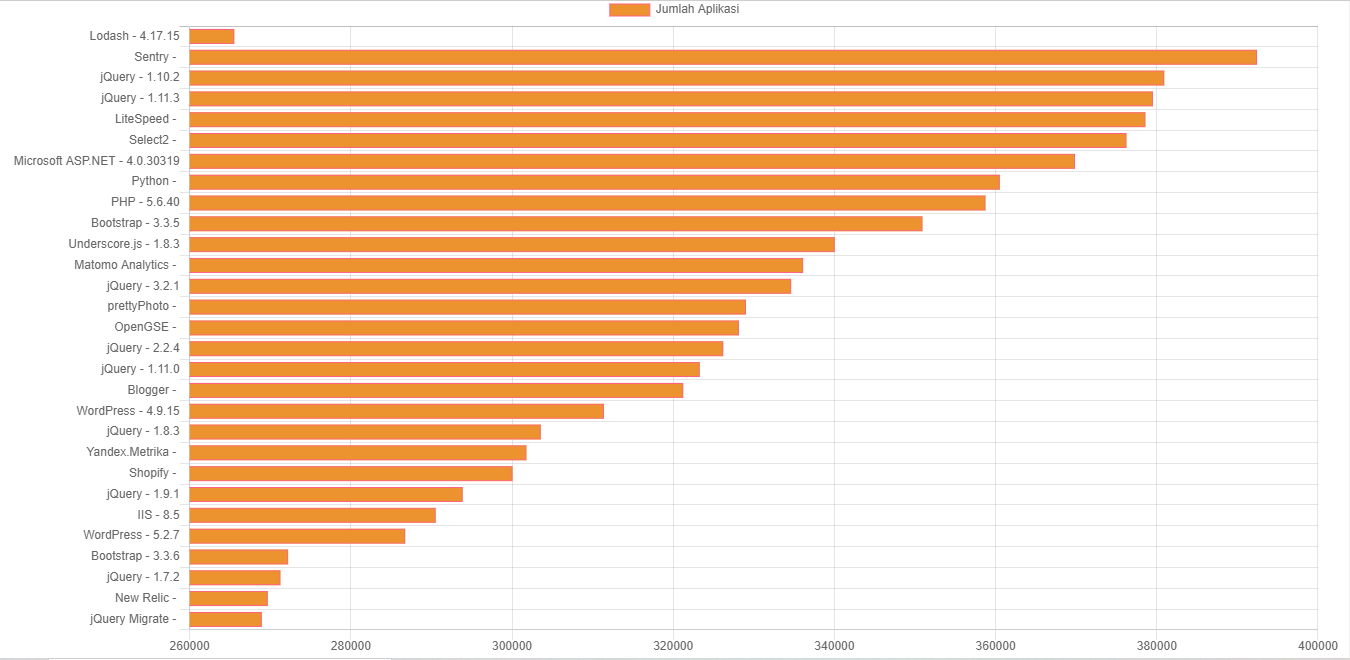
\includegraphics[scale=0.5]{Gambar/hasil_chart_all.PNG}  
\caption{Data Sample Jumlah Aplikasi Dengan Versi yang Dipakai} 
\label{fig:data_sample_res} 
\end{figure}